\documentclass[dvipdfmx,autodetect-engine]{jsarticle}
\usepackage{amsmath}
\usepackage{listings}
\usepackage[dviout]{graphicx}
\usepackage{ascmac}

\usepackage{authblk}
\usepackage[utf8]{inputenc}
\renewcommand{\figurename}{Fig.}

\title{The Documentation of Graph Track in Core Challenge}

\author[1]{Takashima Yuya}
\author[1]{Yamaoka Chuta}
\affil[1]{Minato laboratory of Kyoto University}
\date{31 March 2022}

\begin{document}
\maketitle
\section{Graph Structure}
Consider a piece consisting of $5$ vertices and $2$ tokens (Fig. 1).
This piece can switch between 0-state and 1-state via transition-state as shown in Figure 2.\\
Here, if vertex 1 is blocked by an external token in the 0-state or 1-state state, this piece will not be able to switch states (Fig. 3). 
By preparing piece-1 and piece-2 and connecting them with edges as shown in Figure 4, it is possible to make the possibility of transition of piece-2 depend on piece-1.\\
Prepare $n$ pieces piece-$1$, piece-$2$ $\ldots$ piece-$n$. For $i (2 \le i \le n)$, stretch the edges so that piece-$i$ is transitive only when piece-$i-1$ is 1-state and piece-$j (1 \le j \le i-2)$ is 0-state.
The initial token placement state is such that each piece is 0-state.
The target token placement state is set so that only piece-$n$ is 1-state and all other pieces are 0-state.\\
Suppose there are $m$ pieces, and the state of each piece is represented by an 01-string of length $m$. In the transition from the initial state to the target state, this 01-string changes by one character, and all $2^m$ possible 01-strings are transitioned as in the Gray code.


\section{Reconfiguration Sequence Length}
Each piece requires $3$ transitions to change its state.
There are $|V|/5$ pieces in the graph, therefore the reconfiguration sequence length is $3 \times (2^{|V|/5} - 1)$.

\begin{description}
    \item[10 vertices:] 2 pieces, so the length is $3 \times (2^2 - 1) = 9$.
    \item[50 vertices:] 10 pieces, so the length is $3 \times (2^{10} - 1) = 3069$.
    \item[100 vertices:] 20 pieces, so the length is $3 \times (2^{20} - 1) = 3145725$.
\end{description}


\begin{figure}[b]
  \begin{center}
    \caption{A piece consisting of $5$ vertices and $2$ tokens}
    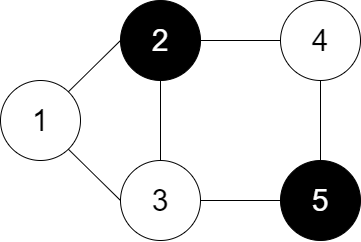
\includegraphics[scale=0.3]{part.png}
    \label{lednum}
  \end{center} 
\end{figure}


\begin{figure}[b]
  \begin{center}
    \caption{Transition of a piece}
    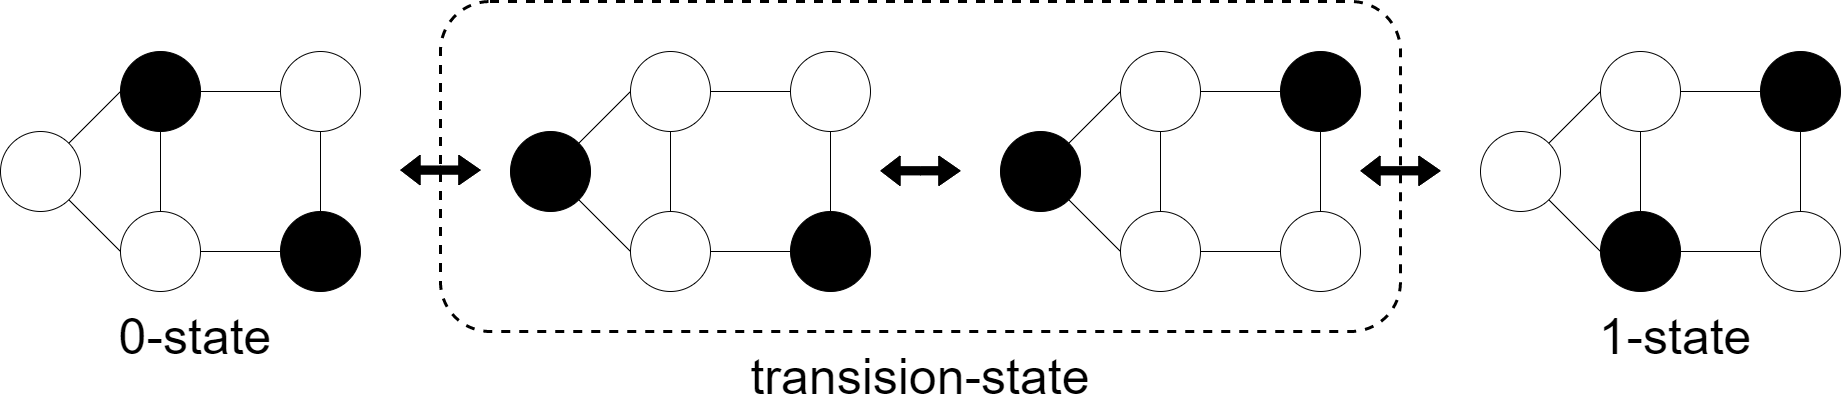
\includegraphics[scale=0.2]{transition.png}
    \label{lednum}
  \end{center} 
\end{figure}


\begin{figure}[b]
  \begin{center}
    \caption{Blocking transitions by external tokens}
    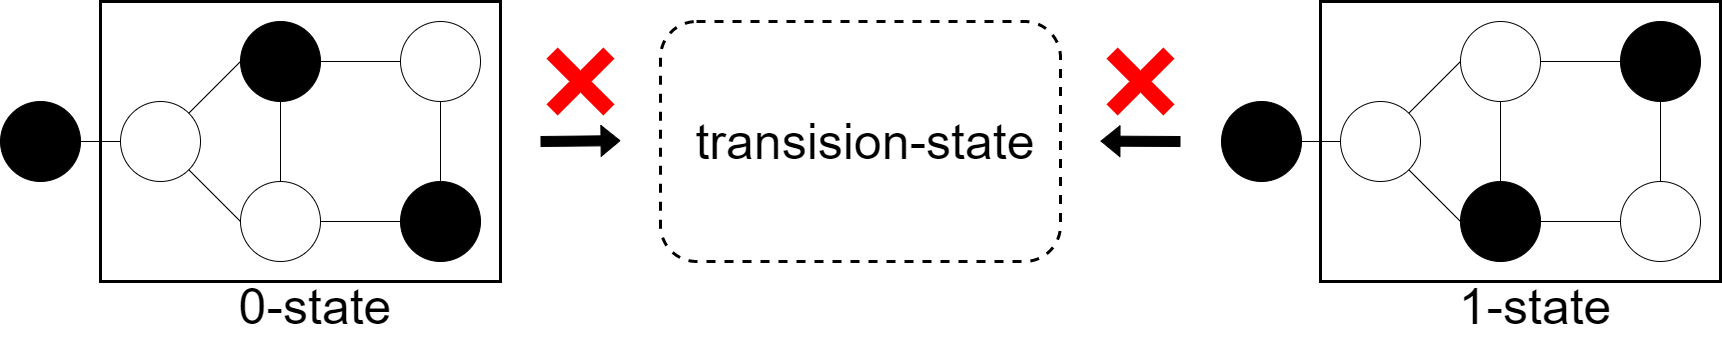
\includegraphics[scale=0.2]{blocking.png}
    \label{lednum}
  \end{center} 
\end{figure}


\begin{figure}[b]
  \begin{center}
    \caption{Blocking transitions depending on the state of the external piece}
    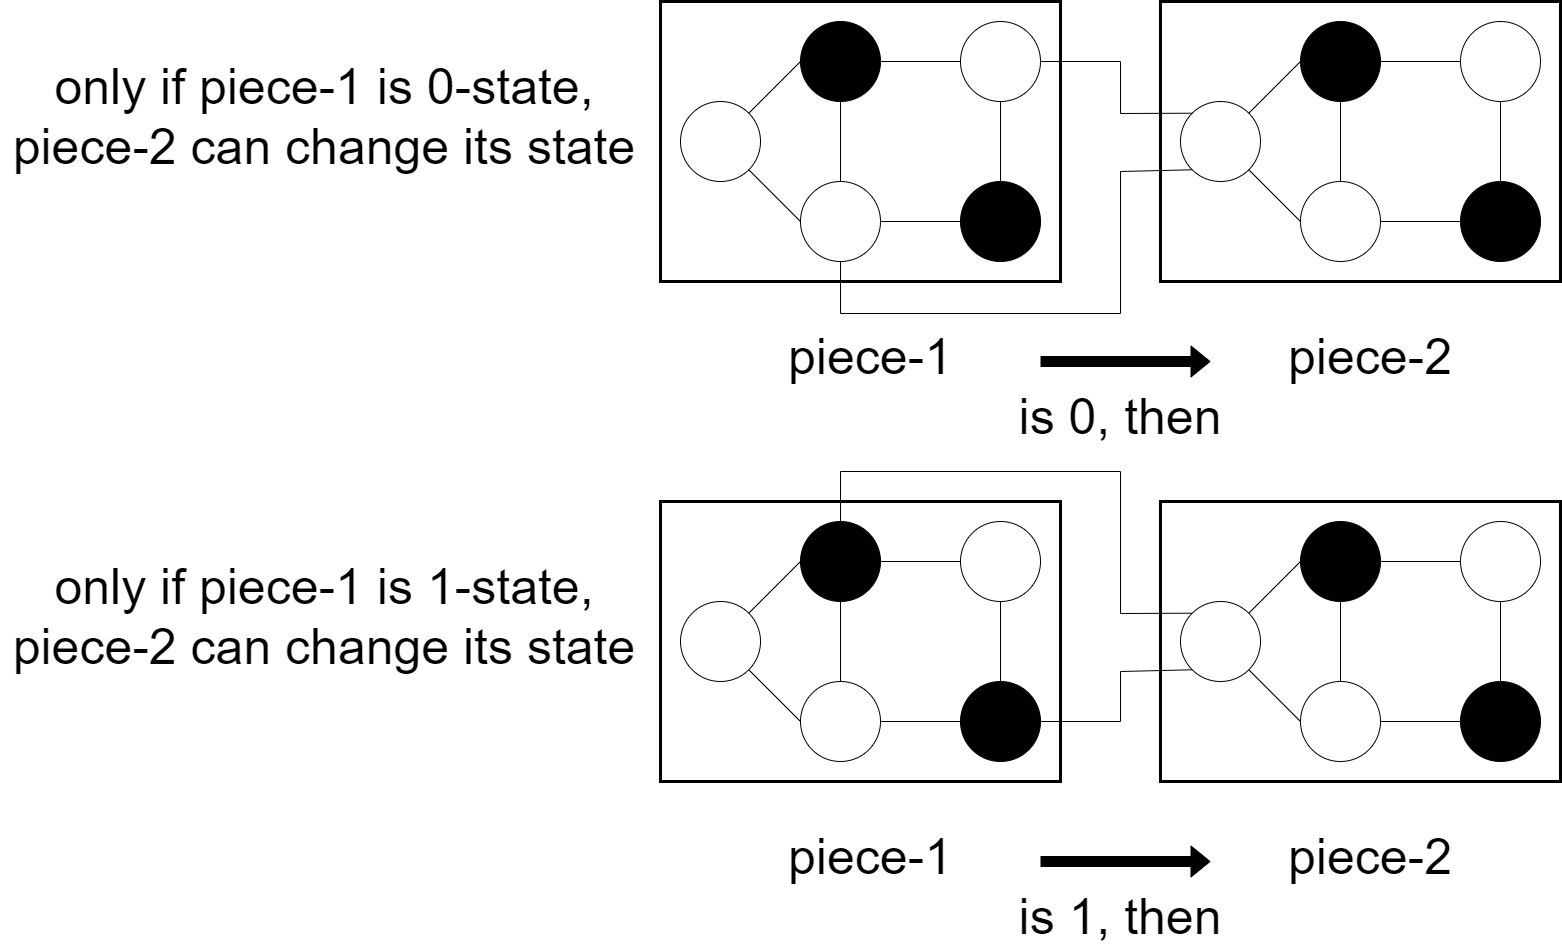
\includegraphics[scale=0.2]{transitionif.png}
    \label{lednum}
  \end{center} 
\end{figure}


\begin{figure}[b]
  \begin{center}
    \caption{Connection of each piece}
    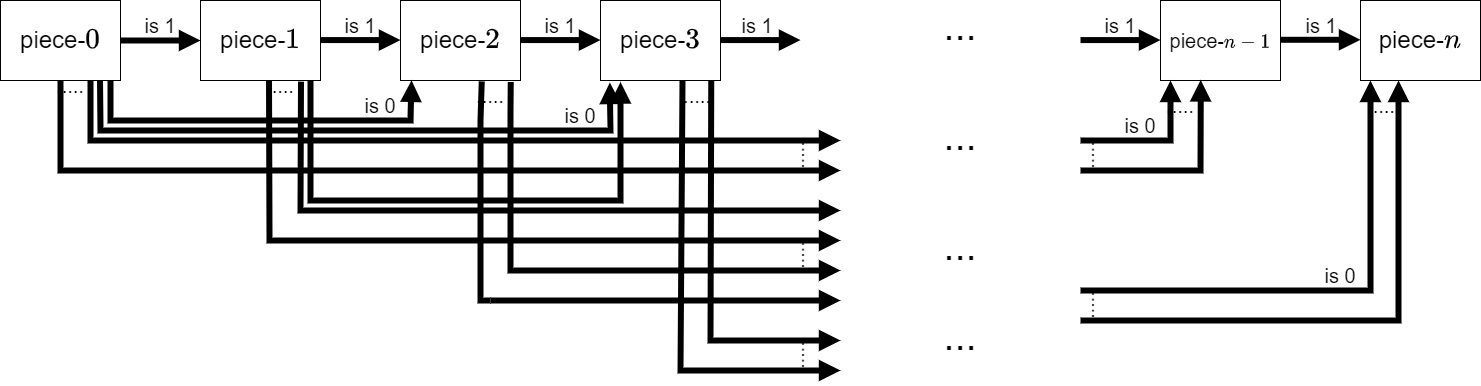
\includegraphics[scale=0.2]{chain.png}
    \label{lednum}
  \end{center} 
\end{figure}

\end{document}